\documentclass[border=10pt]{standalone}
\usepackage{fontspec}
\usepackage{unicode-math}
\setmainfont{PT Sans}
\setmathfont[Path=../, math-style=upright]{Neo Euler.otf}
\usepackage{tikz,pgfplots}
\pgfplotsset{compat=1.17}
\usetikzlibrary{positioning,arrows.meta,calc,decorations.pathreplacing,shapes.geometric}
% палитра manim (3Blue1Brown): оттенки A (светлый) ... E (тёмный); линии — D/E, заливки — A
\definecolor{mBlueA}{HTML}{C7E9F1}
\definecolor{mBlueB}{HTML}{9CDCEB}
\definecolor{mBlueC}{HTML}{58C4DD}
\definecolor{mBlueD}{HTML}{29ABCA}
\definecolor{mBlueE}{HTML}{236B8E}
\definecolor{mTealA}{HTML}{ACEAD7}
\definecolor{mTealB}{HTML}{76DDC0}
\definecolor{mTealC}{HTML}{5CD0B3}
\definecolor{mTealD}{HTML}{55C1A7}
\definecolor{mTealE}{HTML}{49A88F}
\definecolor{mGreenA}{HTML}{C9E2AE}
\definecolor{mGreenB}{HTML}{A6CF8C}
\definecolor{mGreenC}{HTML}{83C167}
\definecolor{mGreenD}{HTML}{77B05D}
\definecolor{mGreenE}{HTML}{699C52}
\definecolor{mYellowA}{HTML}{FFF1B6}
\definecolor{mYellowB}{HTML}{FFEA94}
\definecolor{mYellowC}{HTML}{F7D96F}
\definecolor{mYellowD}{HTML}{F4D345}
\definecolor{mYellowE}{HTML}{E8C11C}
\definecolor{mGoldA}{HTML}{F7C797}
\definecolor{mGoldB}{HTML}{F9B775}
\definecolor{mGoldC}{HTML}{F0AC5F}
\definecolor{mGoldD}{HTML}{E1A158}
\definecolor{mGoldE}{HTML}{C78D46}
\definecolor{mRedA}{HTML}{F7A1A3}
\definecolor{mRedB}{HTML}{FF8080}
\definecolor{mRedC}{HTML}{FC6255}
\definecolor{mRedD}{HTML}{E65A4C}
\definecolor{mRedE}{HTML}{CF5044}
\definecolor{mMaroonA}{HTML}{ECABC1}
\definecolor{mMaroonB}{HTML}{EC92AB}
\definecolor{mMaroonC}{HTML}{C55F73}
\definecolor{mMaroonD}{HTML}{A24D61}
\definecolor{mMaroonE}{HTML}{94424F}
\definecolor{mPurpleA}{HTML}{CAA3E8}
\definecolor{mPurpleB}{HTML}{B189C6}
\definecolor{mPurpleC}{HTML}{9A72AC}
\definecolor{mPurpleD}{HTML}{715582}
\definecolor{mPurpleE}{HTML}{644172}
\colorlet{blue}{mBlueE}
\colorlet{red}{mRedE}
\colorlet{green}{mGreenE}
\colorlet{gold}{mGoldE}
\colorlet{purp}{mPurpleE}
\colorlet{maroon}{mMaroonD}
\colorlet{teal}{mTealE}
\colorlet{yellow}{mYellowE}
\colorlet{skyblue}{mBlueD}
\colorlet{fillblue}{mBlueA}
\colorlet{fillgreen}{mGreenA}
\colorlet{fillred}{mRedA}
\colorlet{fillgold}{mGoldA}
\colorlet{fillpurp}{mPurpleA}
\colorlet{fillteal}{mTealA}
\definecolor{grey}{RGB}{150,150,150}
\tikzset{
  neuron/.style={circle, draw=black, line width=1.2pt, minimum size=11mm, font=\Large, fill=white, inner sep=1pt},
  block/.style={rectangle, draw=black, line width=1.2pt, minimum height=10mm, minimum width=16mm, font=\Large, fill=white},
  opnode/.style={rectangle, rounded corners=3mm, draw=black, line width=1.2pt, minimum height=9mm, font=\Large, fill=white, inner xsep=8pt},
  edge/.style={line width=1.2pt, -{Stealth[length=2.6mm]}, shorten >=1pt},
  plain/.style={line width=1.2pt},
  thinedge/.style={line width=0.6pt, grey},
  wl/.style={font=\large, fill=white, inner sep=1.5pt},
  lbl/.style={font=\large},
  curve/.style={black, line width=1.6pt},
  curveB/.style={blue, line width=1.6pt},
  curveR/.style={red, line width=1.6pt},
  hollow/.style={fill=white, draw=blue, line width=1.2pt},
  regionR/.style={fill=fillred, fill opacity=0.6},
  regionB/.style={fill=fillblue, fill opacity=0.6},
  sep/.style={green, line width=1.4pt, dashed},
  cell/.style={draw=black, line width=0.8pt, minimum size=8mm, font=\large, inner sep=0pt},
}
\pgfplotsset{
  dlgrid/.style={grid=major, grid style={dashed, gray!30}},
  dlaxis/.style={axis lines=middle, axis line style={line width=1.2pt, -{Stealth[length=2.6mm]}},
    tick style={line width=1pt, black}, ticklabel style={font=\large}, label style={font=\large},
    xlabel style={anchor=north west}, ylabel style={anchor=south east}, clip=false},
  cls0/.style={only marks, mark=*, mark size=4pt, mark options={fill=blue, draw=blue}},
  cls1/.style={only marks, mark=x, mark size=5pt, mark options={draw=red, line width=2.2pt}},
}

\begin{document}
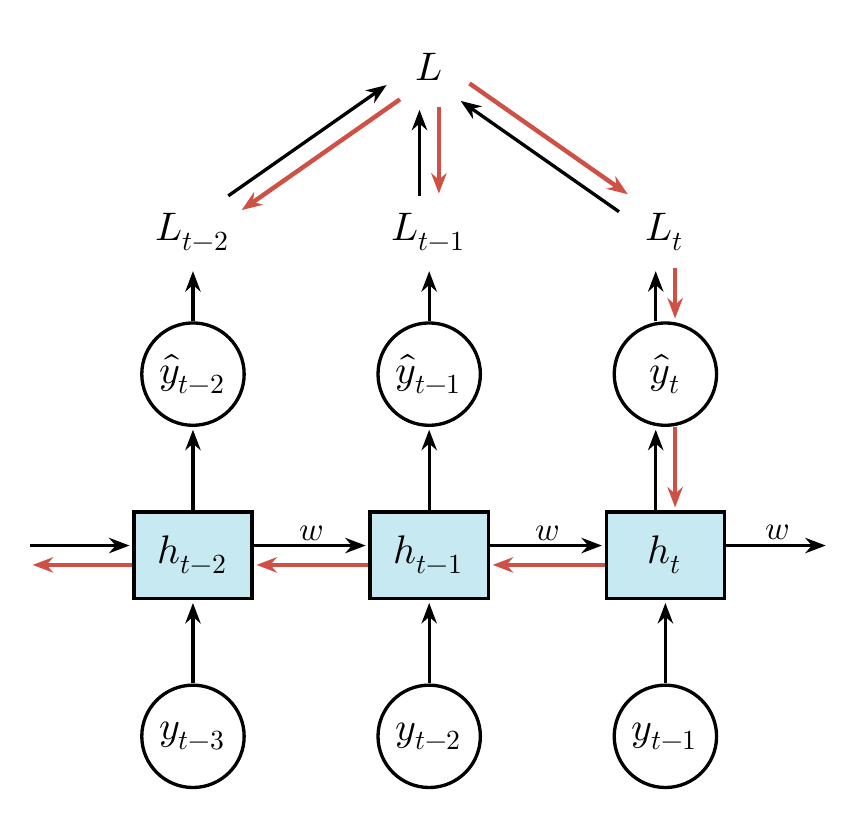
\begin{tikzpicture}
  \tikzset{
    hstate/.style={block, fill=fillblue, minimum width=15mm, minimum height=11mm},
    io/.style={neuron, minimum size=13mm},
    loss/.style={ellipse, font=\Large, inner sep=0pt, minimum width=17mm, minimum height=9mm},
    back/.style={edge, red, line width=1.6pt},
  }
  \def\dx{3}
  \foreach \i/\x/\yin/\yout/\h in {0/0/{y_{t-3}}/{\hat y_{t-2}}/{h_{t-2}}, 1/\dx/{y_{t-2}}/{\hat y_{t-1}}/{h_{t-1}}, 2/2*\dx/{y_{t-1}}/{\hat y_{t}}/{h_{t}}}{
    \node[io] (x\i) at (\x, -2.3) {$\yin$};
    \node[hstate] (h\i) at (\x, 0) {$\h$};
    \node[io] (y\i) at (\x, 2.3) {$\yout$};
    \draw[edge] (x\i) -- (h\i);
  }
  \node[loss] (l0) at (0, 4.1) {$L_{t-2}$};
  \node[loss] (l1) at (\dx, 4.1) {$L_{t-1}$};
  \node[loss] (l2) at (2*\dx, 4.1) {$L_{t}$};
  \node[loss, minimum width=11mm, minimum height=10mm] (sl) at (\dx, 6.2) {$L$};

  \coordinate (in) at ($(h0.west)+(-1.3,0)$);
  \draw[edge] ($(h2.east)+(0,3.5pt)$) -- node[wl, above] {$w$} ($(h2.east)+(1.3,3.5pt)$);

  \draw[edge] (h0) -- (y0);
  \draw[edge] (h1) -- (y1);
  \draw[edge] (y0) -- (l0);
  \draw[edge] (y1) -- (l1);

  \node[wl, above] at ($(h0.east)!0.5!(h1.west)+(0,3.5pt)$) {$w$};
  \node[wl, above] at ($(h1.east)!0.5!(h2.west)+(0,3.5pt)$) {$w$};
  \foreach \p/\q in {in/h0.west, h0.east/h1.west, h1.east/h2.west, h2.north/y2.south, y2.north/l2.south}{
    \coordinate (p) at (\p);
    \coordinate (q) at (\q);
    \draw[edge] ($(p)!3.5pt!90:(q)$) -- ($(q)!3.5pt!-90:(p)$);
    \draw[back] ($(q)!3.5pt!90:(p)$) -- ($(p)!3.5pt!-90:(q)$);
  }

  \foreach \i/\a/\b in {0/35/215, 1/90/270, 2/145/325}{
    \coordinate (p) at (l\i.\a);
    \coordinate (q) at (sl.\b);
    \draw[edge] ($(p)!3.5pt!90:(q)$) -- ($(q)!3.5pt!-90:(p)$);
    \draw[back] ($(q)!3.5pt!90:(p)$) -- ($(p)!3.5pt!-90:(q)$);
  }
\end{tikzpicture}
\end{document}
